\documentclass[xcolor=dvipsnames,handout,t]{beamer}
% use handout in document class to stop transitions

\mode<presentation>
{
  \usetheme{Madrid}%{Madrid}
  % or ..AnnArbor, Boadilla, CambridgeUS, Copenhagen, default, Frankfurt, Goettingen, Hannover
  %       Montpellier, PaloAlto, Rochester, Szeged,

  \setbeamercovered{invisible}
  % or whatever (possibly just delete it)
}
\usepackage{color,empheq}
\usepackage{subfigure}
\usepackage{caption}
\usepackage{subcaption}
\usepackage[english]{babel}
\usepackage{xmpmulti,animate}
\usecolortheme{seahorse} %this makes the colors less strong.

\usepackage{times}
% Or whatever. Note that the encoding and the font should match. If T1
% does not look nice, try deleting the line with the fontenc.
\usepackage{graphicx}
%\usepackage{tcolorbox}
\usepackage{tikz,lipsum,lmodern}
\usepackage[most]{tcolorbox}
\usepackage{amsfonts,amssymb,amsmath,mathtools}
      % use Times fonts if available on your TeX system
\usepackage{epsfig}
\usepackage{hyperref}
\usepackage{changepage}
\usepackage[utf8]{inputenc}
\usepackage[T1]{fontenc}
%\usepackage{animate,movie15,media9}
%\usepackage{multimedia}

\newcommand{\todo}[1]{\textcolor{orange}{\texttt{TODO: #1}}} 
\newcommand{\red}[1]{\textcolor{red}{#1}} 
\newcommand{\bl}[1]{\textcolor{blue}{#1}} 


\usetikzlibrary{shapes}

\title[] % (optional, use only with long paper titles)


%\subtitle
%{Presentation Subtitle} % (optional)

\title[Forecasting GRBs w/ GWs] % (optional, use only with long paper titles)
{Forecasting Gamma-ray Bursts with Gravitational Waves}

\subtitle{\todo{Add background image}} % (optional)

\author[Sarp Akcay]{Sarp Akcay\inst{1}\inst{2} }
\institute[FSU Jena - UCD] % (optional, but mostly needed)
{
  \inst{1}%
  FSU Jena %and University College Dublin
  \inst{2}%
  University College Dublin
  }


%\vspace{-3cm}
%\titlegraphic{
%  \vspace{1.75cm}  \includegraphics[width=1.0cm]{figs/ucd.png}%\hspace*{1cm}~\includegraphics[height=1cm]{figs/missing_inch.jpg} \hspace*{1cm}  \includegraphics[width=1.0cm]{figs/ucd.png}
%}
\date[Sabanci University]{14 November 2018}

\subject{Talks}

\usefonttheme[onlymath]{serif}
\setbeamerfont{frametitle}{size=\huge}
\setbeamercolor{frametitle}{fg=Black,bg=White}

\newcommand{\Mag}{\textcolor{magenta}}
\newcommand{\Red}{\textcolor{red}}
\newcommand{\Blue}{\textcolor{blue}}
\renewcommand{\c}{\cos}
\renewcommand{\t}{\theta}
\renewcommand{\b}{\bar}
\newcommand{\f}{\frac}
\newcommand{\bt}{\beta}
%\newcommand{\s}{\sin}
\newcommand{\ph}{\phi}
\newcommand{\g}{\gamma}
\newcommand{\nn}{\nonumber}
\newcommand{\la}{\lambda}
\newcommand{\al}{\alpha}
\newcommand{\La}{\Lambda}
\newcommand{\el}{\ell}
\newcommand{\h}{\hat}
\newcommand{\mrm}{\mathrm}
\newcommand{\ord}{\mathcal{O}}
\newcommand{\F}{\mathcal{F}}
\newcommand{\be}{\begin{equation}}
\newcommand{\ee}{\end{equation}}
\newcommand{\ba}{\begin{eqnarray}}
\newcommand{\ea}{\end{eqnarray}}
\newcommand{\bi}{\begin{itemize}}
\newcommand{\ei}{\end{itemize}}
\newcommand{\bef}{\begin{frame}}
\newcommand{\ef}{\end{frame}}
%\newcommand{\h}{\bar{h}}
\newcommand{\bs}{\begin{small}}
\newcommand{\es}{\end{small}}
\newcommand{\parallelsum}{\mathbin{\!/\mkern-5mu/\!}}
\newcommand{\Lim}[1]{\raisebox{0.5ex}{\scalebox{0.8}{$\displaystyle \lim_{#1}\;$}}}
\newcommand*\circled[1]{\tikz[baseline=(char.base)]{\node[shape=circle,draw,inner sep=2pt] (char) {#1};}}
%------------------ for coloured boxes in math modes --------------------
% Syntax: \colorboxed[<color model>]{<color specification>}{<math formula>}
\newcommand*{\colorboxed}{}
\def\colorboxed#1#{%
  \colorboxedAux{#1}%
}
\newcommand*{\colorboxedAux}[3]{%
  % #1: optional argument for color model
  % #2: color specification
  % #3: formula
  \begingroup
    \colorlet{cb@saved}{.}%
    \color#1{#2}%
    \boxed{%
      \color{cb@saved}%
      #3%
    }%
  \endgroup
}
%%-------------------------------------------------------------------------

% tikz boxes
\newcommand\TBox[3][]{%
  \tikz\node[draw,ultra thick,red,text width=#2,align=left,#1] {#3};}

\setbeamertemplate{frametitle}[default][center]



\begin{document}
%{
%\usebackgroundtemplate{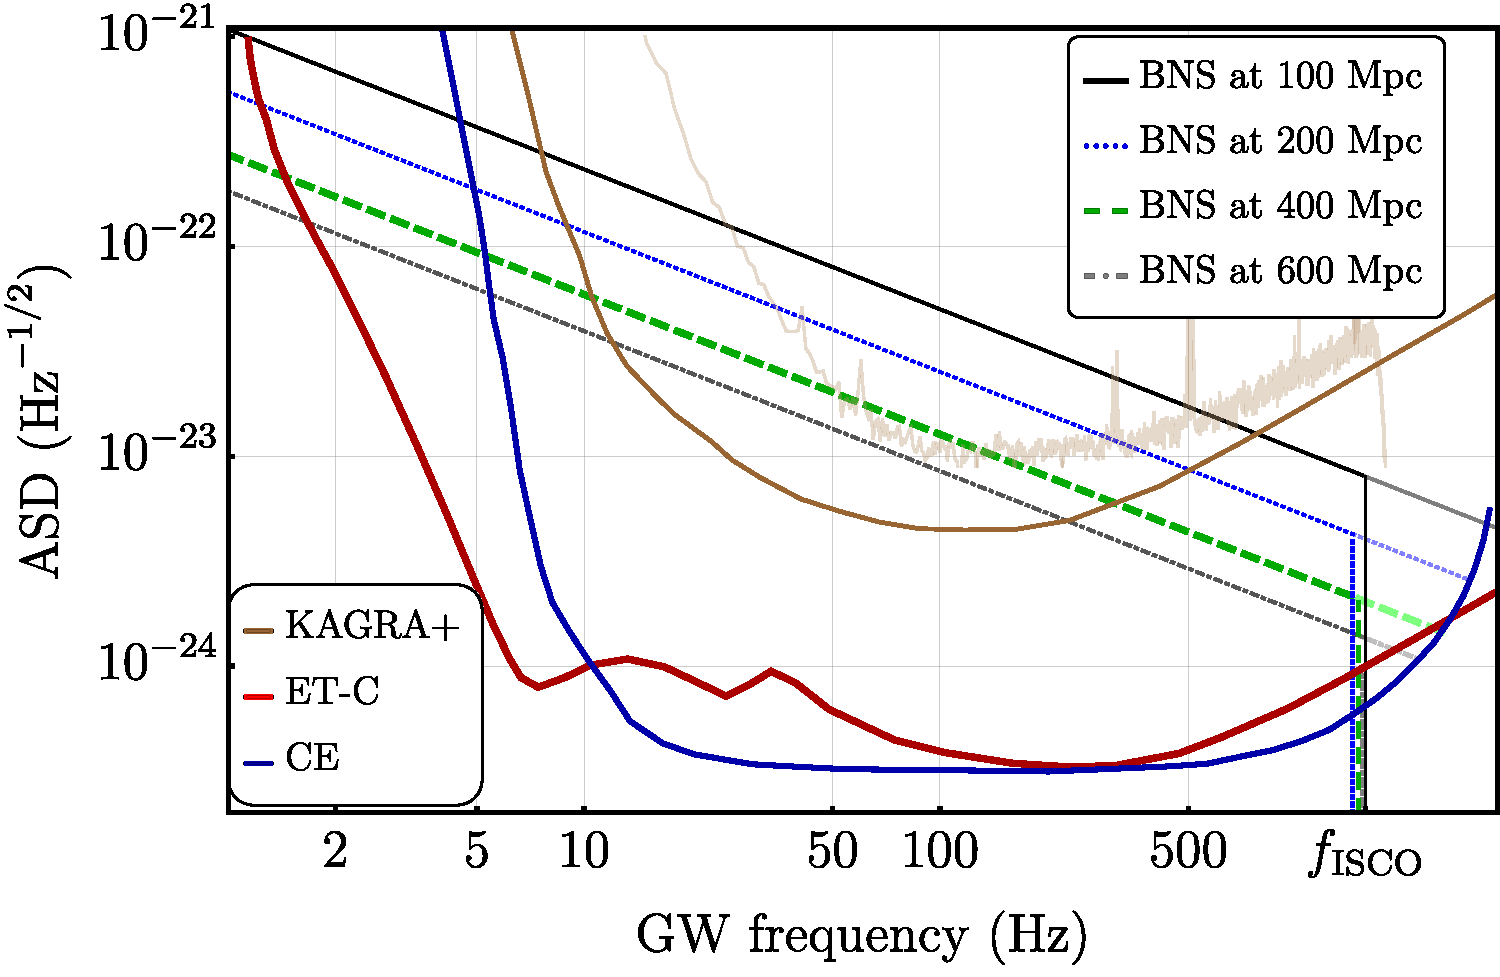
\includegraphics[width=1\paperwidth,height=\paperheight]{../Figures/ET_strains_redshifted_v2.pdf}}
\begin{frame}
 \titlepage
\end{frame}
%}

\begin{frame}{Outline}
\begin{itemize}
 \item Motivation
 \item Gravitational waves
 \item Binary neutron star inspirals
 \item Gravitational-wave detectors
 \item Event rates 
\end{itemize}
\todo{finish this slide remove later if short on time}

 
\end{frame}


\begin{frame}{Motivation: Multi-messenger Astronomy}
\begin{itemize}
 \item \emph{Multi}: two fundamentally different waves from common events.
 \item[]\quad Gravitational waves (GWs): ``hearing''  the universe.
 \item[]\quad Electromagnetic waves (EWs): ``seeing'' the universe.
 \item \red{GW170817}-\bl{GRB170817A}-\textcolor{brown}{AT2017gfo}: the ``event'' \\
 \quad inspiral + merger of two neutron stars (GWs) \\
 \ \ = short-hard gamma-ray burst + kilonova (EWs)
 \item[] Broad-band in gravitational waves: 10Hz - 2000Hz
 \item[] Ultra broad-band in electromagnetic waves: gamma rays to radio.
 \item A simple question \\
{\small ``What can we offer to the astronomy community with future GW detections?''}
 \end{itemize}


 \end{frame}

 
\begin{frame}{Gravitational waves: Einstein 1916}
  \begin{center}
\begin{tikzpicture}
            \node[anchor=south west,inner sep=0] at (0,0) {\includegraphics[height=3.5cm]{figs/Einstein1916.png}};
            %\draw<1>[red,ultra thick,rounded corners] (1.6,1) rectangle (\textheight-1cm,5);
           \uncover<3->{\draw<3->[red,thick] (1.7,0.04) rectangle (3.1,0.27);}
        \end{tikzpicture}
        \\
         \uncover<2->{Perturbations of spacetime with speed $=c$, sourced by accelerating masses.}
         \end{center}
          \begin{itemize}
 \item  \uncover<3->{Spacetime metric $g_{\mu\nu} = \eta_{\mu\nu} + h_{\mu\nu}$, \quad with $| h_{\mu\nu} | \ll 1$.}
 \item  \uncover<4->{Insert into $G_{\mu\nu} = 0$. Keep only $\mathcal{O}(h)$. Pick a gauge.} %(e.g. Lorenz).}
  \uncover<5->{\[ \Rightarrow\quad \Box \bar{h}_{\mu\nu}= 0, \quad \text{wave equation!} \]}
  \item \uncover<6->{\alert{Plane-waves:} $ \bar{h}_{\mu\nu} = \Re\left[A_{\mu\nu}\, \text{e}^{i k_\mu x^\mu}\right] =\Re\left[A_{\mu\nu}\, \text{e}^{-i\omega (t-z/c )}\right]$.}
 \end{itemize}
\end{frame}

\begin{frame}{Gravitational waves: d.o.f.'s}
$A_{\mu\nu} $ is the polarization tensor.
\begin{itemize}
 \uncover<2->{\item $\{ \bar{h}_{\mu\nu}, A_{\mu\nu} \}$: $4\times4$, symmetric \uncover<3->{$\hspace{1.5cm}\Rightarrow \f{4\times 5}{2}\ \ \ = 10$ d.o.f.}}
 \uncover<4->{\item Gauge condition: $\nabla_\mu \bar{h}^{\mu\nu} =  A_{\mu\nu} k^\nu= 0$ \uncover<5->{$\Rightarrow10-4 = \, 6$ d.o.f.}}
 \uncover<6->{\item Residual gauge freedom \hspace{2.25cm} \uncover<7->{$\Rightarrow 6-4 \ \ = \alert{2}$ \alert{d.o.f.}}}
 %\uncover<7->{\vspace{2mm}\begin{center}$ \bar{h}'_{\mu\nu} = \bar{h}_{\mu\nu} - \xi_{\mu,\nu} - \xi_{\nu,\mu} + \eta_{\mu\nu} \nabla_\alpha \xi^\alpha . $ \end{center}\vspace{2mm}}
\end{itemize}
\uncover<7->{\quad \ Consistent with $\pm 2$ helicities of a \bl{massless} spin 2 boson.\\}
\uncover<8->{$\Rightarrow$ \alert{2} POLARIZATIONS (\alert{transverse}): \uncover<10->{$\begin{array}{l}A_{xx}=-A_{yy} = \red{h_+}  \\ A_{xy}=\ \ A_{yx} = \red{h_\times}  \\ \end{array}$}}
\\
\todo{Replace with Maggiore's discussion?}
{\begin{center} \includegraphics[height=2.79875cm]{figs/white_box.png}\end{center}}
\end{frame}
 
 

\begin{frame}{Gravitational waves: d.o.f.'s}
%\begin{center}
%\animategraphics[loop,controls,width=3cm]{12}{GWs_frame-}{0}{29} 
%\end{center}
$A_{\mu\nu} $ is the polarization tensor.
\begin{itemize}
{\item $\{ \bar{h}_{\mu\nu}, A_{\mu\nu} \}$: $4\times4$, symmetric {$\hspace{1.5cm}\Rightarrow \f{4\times 5}{2}\ \ \ = 10$ d.o.f.}}
 {\item Gauge condition: $\nabla_\mu \bar{h}^{\mu\nu} =  A_{\mu\nu} k^\nu= 0${ $\Rightarrow10-4 = \,6$ d.o.f.}}
 {\item Residual gauge freedom \hspace{2.25cm}{ $\Rightarrow 6-4 \ \ = \alert{2}$ \alert{d.o.f.}}}
 %{\vspace{2mm}\begin{center}$ \bar{h}'_{\mu\nu} = \bar{h}_{\mu\nu} - \xi_{\mu,\nu} - \xi_{\nu,\mu} + \eta_{\mu\nu} \nabla_\alpha \xi^\alpha . $ \end{center}\vspace{2mm}}
\end{itemize}
{\quad \ Consistent with $\pm 2$ helicities of a \bl{massless} spin 2 boson.\\}
{$\Rightarrow$ \alert{2} POLARIZATIONS (\alert{transverse}): {$\begin{array}{l}A_{xx}=-A_{yy} = \red{h_+}  \\ A_{xy}=\ \ A_{yx} = \red{h_\times}  \\ \end{array}$}}
\\
\todo{Replace with Maggiore's discussion?}
{\begin{center} \animategraphics[loop,controls,height=2.4cm]{12}{GWs_plus-}{0}{20} \hspace{1cm} \animategraphics[loop,controls,height=2.4cm]{12}{GWs_cross-}{0}{20}\end{center}}
\end{frame}

\begin{frame}{Making gravitational waves}{non-spherical, accelerated motion}
 \alert{Inspirals}, GRBs, bumps on neutron stars, supernovae, the Big Bang. \\% (BICEP 2).\\
 \uncover<2->{Gravitational-wave luminosity: \uncover<3->{\alert{quadrupole} radiation}  (leading-order)}
 \uncover<3->{\begin{center} $ \boxed{\dot{E}=L_\text{GW} = \f{G}{c^5} \langle (\partial_t^3 \bar{Q}_{ij})^2 \rangle}$\\\vspace{2mm}}
 \uncover<4->{\begin{small}$ \quad \bar{Q}_{ij} = Q_{ij}-\frac{1}{3}\delta_{ij}Q^k_k, \quad Q^{ij} = \int \rho(t,{\mathbf x})x^i x^j d^3 x $ \end{small} \end{center}}
 \uncover<5->{{\bf Binary systems:} 2 points masses in circular orbit. }
 
\end{frame}

\begin{frame}{Making gravitational waves}{non-spherical, accelerated motion}
 \alert{Inspirals}, GRBs, bumps on neutron stars, supernovae, the Big Bang. \\%  (BICEP 2).\\
 Gravitational-wave luminosity: \alert{quadrupole} radiation (leading-order)
 \begin{center} $ \boxed{\dot{E}=L_\text{GW} = \f{G}{c^5} \langle (\partial_t^3 \bar{Q}_{ij})^2 \rangle}$\\ \vspace{2mm}
 \begin{small}$ \quad \bar{Q}_{ij} = Q_{ij}-\frac{1}{3}\delta_{ij}Q^k_k, \quad Q^{ij} = \int \rho(t,{\mathbf x})x^i x^j d^3 x $ \end{small} \end{center}
 {\bf Binary systems:} 2 points masses in circular orbit.\todo{$R\to r$ in vid}
 \begin{tikzpicture}[overlay,remember picture]
\onslide<5->\node (img0 )[anchor=center,scale=1,opacity=1] at ([shift={(-3.8cm,-2.8cm)}]current page.center) {\animategraphics[loop,controls,height=2.4cm]{12}{Circ_Orb-}{0}{20}};
\onslide<2->\node (t1 )[anchor=center,scale=1,opacity=1] at ([shift={(2cm,-1.3cm)}]current page.center) {$\mu=m_1 m_2/M^2,\ x(t) = r \cos\Omega t, \ y(t) = r \sin\Omega t $};
\onslide<3->\node (t2 )[anchor=center,scale=1,opacity=1] at ([shift={(2.25cm,-2.2cm)}]current page.center) {$ Q^{ij} =  2 M\, x^i x^j, \qquad \boxed{\dot{E} = \f{32}{5}\f{G\mu^2}{c^5}r^4 \Omega^6}$};
\onslide<4->\node (t3 )[anchor=center,scale=1,opacity=1] at ([shift={(2.5cm,-3.2cm)}]current page.center) {Enhancement due to \bl{$e$} (Peters \& Mathews).};
\onslide<5->\node (t3 )[anchor=center,scale=1,opacity=1] at ([shift={(2cm,-4cm)}]current page.center) {$ \bl{\f{\left(1 + \f{73}{24}e^2+ \f{37}{96} e^4 \right)}{(1-e^2)^{7/2}}}$};
\end{tikzpicture}
\end{frame}








 \begin{frame}{Compact Binary Inspirals}
 Notation:
 \begin{itemize}
  \item $\red{f} $: GW frequency, \hspace{1.5cm} $\Longrightarrow\quad \omega\equiv2\pi f = 2\Omega$.
  %\item $\omega\equiv2\pi f = 2\Omega$: GW angular frequency.
  \item $t$: observer/detector time \quad$ \Longrightarrow\quad\dot{Y}= dY/dt$.
 \end{itemize}

  Assumptions:
  \begin{itemize}
   \item Quasi-circular orbits: $e \ll 1$ and $\tfrac{|\dot{r}|}{r\Omega} <10^{-3} $ at $f=100\,$Hz.
   \item Quadrupolar GWs only: higher modes suppressed by $\tfrac{m_1-m_2}{M}\tfrac{v^2}{c^2}$
   \item Use Newtonian/post-Newtonian theory ($\le$3.5{\bf PN}).
   \item Terminate inspiral at Schwarzschild ISCO \todo{add ISCO curve?}
   \begin{footnotesize}
   \[f_\text{ISCO} = \f{c^3}{6^{3/2}\pi G M} \simeq 1571\,\text{Hz}\, \left(\f{2.8M_\odot}{M}\right)\] 
   \end{footnotesize}
   \end{itemize}
   %
   For binary neutron stars ({\bf BNS})
   \begin{itemize}
   \item Point masses: tidal effects for $f \gtrsim 100\,$Hz
   \item Set $m_1 =m_2 = 1.4 M_\odot$, constraints: $1.2 M_\odot \lesssim m_\text{NS}\lesssim 1.6M_\odot$.
   \item Neglect spins: spin-orbit $\tfrac{\dot{E}_\text{SO}}{\dot{E}} \sim \tfrac{v_s}{c}\tfrac{v}{c}\tfrac{R_\text{NS}}{r}$, spin-spin $\sim \tfrac{v^4}{c^4}$
   \end{itemize}
  

 \end{frame}


\begin{frame}{Compact Binary Inspirals}{Newtonian evolution}
 Define \bl{chirp mass} \hspace{1.cm} $\red{M_c} \equiv \mu^{3/5} M^{2/5} = \tfrac{(m_1 m_2)^{3/5}}{(m_1+m_2)^{1/5}}$ \\
 %and symmetric mass ratio\qquad $\nu \equiv \tfrac{\mu}{M} =\tfrac{m_1 m_2}{M^2}$\\
 \vspace{1mm}
 which gives, using Kepler's \bl{third law}: $\Omega^2 = G M r^{-3}=\omega^2/4$   
 \begin{footnotesize}
  $$ \boxed{\dot{E} = \f{32}{5}\f{c^5}{G} \left(\f{G M_c\, \omega}{2c^3}\right)^{10/3}}$$
 \end{footnotesize}\\
%
{\bf Key idea:} \red{energy balance} between $\dot{E}$ and $\dot{E}_b$\\
 %of gravitational binding energy
\quad where $ E_b= -\tfrac{G m_1 m_2}{2r} = -\left(\tfrac{G^2 M_c^5 \omega^2}{32}\right)^{1/3} $
%
\[ 
 \dot{E}(f) = -\dot{E}_b(f) \Longrightarrow \boxed{\red{\dot{f}} = \f{96}{5}\pi^{8/3} \f{(G M_c)}{c^5}^{5/3}\, \red{f^{11/3}} }
 \]
\[
 \red{ \dot{f} \propto f^{11/3}\quad(1)}
\]

\begin{tikzpicture}[overlay,remember picture]
\node[draw, red,thick,minimum width=3cm,minimum height=0.75cm] (b) at (5.9,0.85){};
\end{tikzpicture}

\end{frame}

\begin{frame}{Compact Binary Inspirals}{Inspiral time \todo{Add $r(t)$ plot? }}
Integrate $\dot{f} \sim f^{11/3} \quad \Longrightarrow \quad \int dt \sim \int f^{-11/3}df \quad\Rightarrow\quad t \sim \red{f^{-8/3}}$
\\
\vspace{1mm}
Fix integration constant $\tau = t_\text{coal} - t >0$. \\
\vspace{2mm}
Introduce \red{inspiral time}, i.e, time to BNS \bl{coal}escence
%
\begin{align}
 \red{\tau_\text{insp}(f)} %&= \f{5}{256\pi}\f{c^5}{(\pi G M_c)^{5/3}} \,{f^{-8/3}}\nn\\
 &\simeq \bl{16.72\,\text{minutes}} \, \left(\f{1.219 M_\odot}{M_c}\right)^{5/3}\,{\left(\f{10\,\text{Hz}}{\red{f}}\right)^{\red{8/3}}\quad \red{(2)}}\nn
\end{align}
Number of GW cycles to coalescence: $\int \tfrac{f}{\dot{f}}df\sim \red{f^{-5/3}}$ %$\int df {f}/\dot{f}$
\begin{align}
 \red{\mathcal{N}_\text{cyc}(f)} %&=\f{1}{32\pi} \f{c^5}{(\pi G M_c)^{5/3}}\left[ f^{-5/3}-f_\text{max}^{-5/3}\right]\nn \\
 &\approx 1.605\times \bl{10^4}\,\left(\f{1.219 M_\odot}{M_c}\right)^{5/3}{ \left(\f{10\,\text{Hz}}{\red{f}} \right)^{\red{5/3}}}\quad \red{(3)}\nn
\end{align}
%
\begin{tikzpicture}[overlay,remember picture]
\node[draw, red,thick,minimum width=8.2cm,minimum height=1.3cm] (b) at (7.,3.35){};
\node[draw, red,thick,minimum width=10cm,minimum height=1.3cm] (b) at (6.2,1){};
\end{tikzpicture}
%
\[ 
\tfrac{\dot{r}}{r}\sim \tfrac{\dot{f}}{f} \Longrightarrow \red{r(\tau)}=r_i \left(\f{\red{\tau}}{\tau_i}\right)^{\red{1/4}}
\]

\end{frame}

\begin{frame}{Gravitational waves from BNS}
TT gauge, multipole, slow-velocity expansions give \todo{add suppl. slide}
\begin{small}
\[
 h_{ij}^\text{TT} = \tfrac{2}{D}\tfrac{G}{c^4} \ddot{Q}_{ij}^\text{TT}%(t-z/c)
\]
%
 \begin{align*}
 h_+(t) &= h_c(t)\, \left(\f{1+\cos^2\iota}{2}\right)\, \cos[\Phi(t)],\\
 h_\times(t) & =h_c(t)\,\cos\iota \sin[\Phi(t)],
\end{align*}
\end{small}
%
%
$\iota =\,$ orbital \bl{inclination}, and
\vspace{-3mm}
%
\begin{small}
\begin{align*}
h_c(t) %&=\f{4}{D}\left(\f{G M_c}{c^2}\right)^{5/3}\, \left(\f{\pi f(t)}{c}\right)^{2/3}\nn\\
&\approx 1.9\times \bl{10^{-23}} \left(\f{40\,\text{Mpc}}{D}\right)\left(\f{M_c}{1.219 M_\odot}\right)^{5/3}\left(\frac{\red{f}}{10\,\text{Hz}}\right)^{\red{2/3}} \nn\\
\Phi(t) &=\int_{t_i}^t dt' \omega(t') + \text{PN corrections}
\end{align*}
\end{small}\\
%
Frequency increases as $f^{11/3}$\\
Amplitude increases as $f^{10/3} \Longrightarrow$ \red{Chirp!} \todo{Insert chirp movie}

\end{frame}



 \begin{frame}{GW Detectors: \red{Interferometers}}
  Two geodesics separated by $\xi^\mu$:
  %\[
  % \frac{D^2 \xi^\alpha}{D\tau^2} = -R^\alpha_{\beta \gamma\delta}\, \xi^\gamma u^\beta u^\delta 
  %\]
$ \tfrac{d^2 \xi^i}{d\tau^2} = -R^i_{0j0} \xi^j\left(\tfrac{dx^0}{d\tau}\right)^2$ \hfill (detector frame)\\
%\hspace{4cm} $\Longrightarrow \ddot{\xi^i} = -c^2 R^i_{0j0} \xi^j $ \hfill (detector time)\ \\
\vspace{-3mm}
\[
\hspace{4.5cm} \boxed{\ddot{\xi^i} = \frac{1}{2} \ddot{h}_{ij}^\text{TT} \xi^j} \hspace{2.5cm} \text{(detector time)}
\]
%
%
GW along $\mathbf{z}$: 
\[
 h_{ij}^\text{TT} = \left(\begin{array}{cc}
                           h_+ & h_\times \\
                           h_\times & - h_+
                          \end{array}\right) \cos\left(\omega\left( t-\tfrac{z}{c}\right)\right)
\]
Consider mirrors at $(0,0)_1, (L,0)_2$ and $(L,L)_3$
\begin{small}
\begin{align*}
  s_{12} &= \int_1^2 \tfrac{ds}{dx}dx = (x_2-x_1) \left[ 1 + h_+ \cos(\omega t)\right]^{1/2}\hspace{4cm} \\
			      & \approx L \left[ 1+\tfrac{1}{2} h_+ \cos\omega t \right] \\
s_{13} &\approx L \left[ 1-\tfrac{1}{2} h_+ \cos\omega t \right]
\end{align*}
\end{small}
%
\begin{tikzpicture}[overlay,remember picture]
%\node (img0 )[anchor=center,scale=1,opacity=1] at ([shift={(3.8cm,-2.8cm)}]current page.center) {\animategraphics[loop,controls,height=2.39cm]{12}{LIGO_int-}{0}{102}};
\end{tikzpicture}
 \end{frame}
 
 

\begin{frame}{Interferometers : \red{L}-topology}{LIGO, Virgo, KAGRA}
\vspace{-2mm}
  Interferometers ({\bf IFO}s) measure only the response function (\bl{GW strain})
  \begin{footnotesize}
  \begin{align*}
   h(t) &= F_+(\theta,\phi,\psi) \,h_+(t)+F_\times(\theta,\phi,\psi)\, h_\times(t) , \\
    F_+ &=\f{1}{2}\left(1+\cos^2\theta\right)\cos2\phi\cos 2\psi-\cos\theta \sin2\phi \sin2\psi, \\
    F_\times &=\f{1}{2}\left(1+\cos^2\theta\right)\cos2\phi\sin2\psi+\cos\theta \sin2\phi \cos2\psi
    \end{align*}
    \end{footnotesize}
   %
   Fourier transform to frequency domain 
  \begin{footnotesize}
  \begin{align*}
  &\red{\tilde{h}(f)} =A\, \underbrace{\f{c}{D}\left(\f{G M_c}{c^3}\right)^{5/6}}_{\bl{h_0}} \,\red{f^{-7/6}}\, e^{i\Psi}\, Q(\theta,\phi,\psi,\iota),\hspace{5cm} \\
     &\quad Q(\theta,\phi,\psi,\iota) = F_+\f{1+\cos^2\iota}{2}  + i F_\times \cos\iota \\
   &\quad A\equiv \pi^{-2/3}\sqrt{\tfrac{5}{24}}\\
   &\quad \Psi = \Psi_N(f) + \text{PN corrections}
    \end{align*}
    \end{footnotesize}
   \red{Four} angles: $\{\theta,\phi,\iota,\psi \}$
   %
  \begin{tikzpicture}[overlay,remember picture]
  \node (img0 )[anchor=center,scale=1,opacity=1] at ([shift={(3.8cm,-1.8cm)}]current page.center) {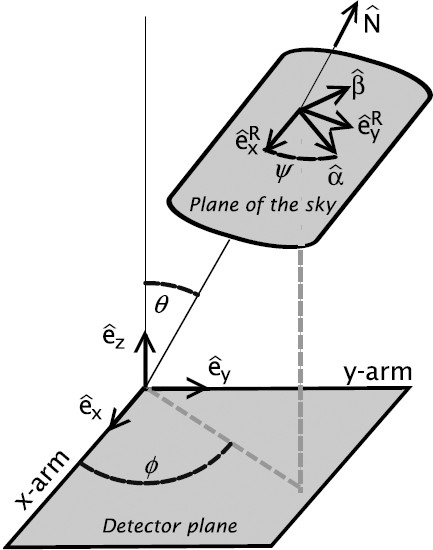
\includegraphics[height=5cm]{figs/Schutz_LRR_Fig3_half.jpg}};
  \end{tikzpicture}
   
\end{frame}


\begin{frame}{Interferometers : \red{Triangular}-topology}{Einstein Telescope}
\vspace{-2mm}
  Three $60^\circ$ V-IFOs, one redundant (null stream), $\sin 60^\circ =\sqrt{3}/2$.
  \begin{footnotesize}
  \begin{align*}
    &F^1_+(\theta,\phi,\psi)= \f{\sqrt{3}}{2} F_+(\theta,\phi,\psi), \qquad F^1_\times(\theta,\phi,\psi)= \f{\sqrt{3}}{2} F_\times(\theta,\phi,\psi),\hspace{2cm}\\
    & F^2_{+,\times}(\theta,\phi,\psi) = F^1_{+,\times}(\theta,\phi+2\pi/3,\psi)\qquad (\text{rotation by 120}^\circ),\\
    & F^3_{+,\times}(\theta,\phi,\psi) = F^1_{+,\times}(\theta,\phi-2\pi/3,\psi) \qquad(\text{rotation by 240}^\circ),\\
    &  |Q(\theta,\phi,\psi,\iota)|_\bigtriangleup^2 = \sum_{A=1}^3 \left(F^A_+\right)^2\f{1+\cos^2\iota}{2}  + \left(F^A_\times\right)^2 \cos\iota
    \end{align*}
    \end{footnotesize}
   %
   No blind spots!
   \begin{footnotesize}
  \begin{align*}
   F^2_\bigtriangleup &\equiv \sum_{A=1}^3 \left(F^A_+\right)^2+\left(F^A_\times\right)^2 \hspace{8cm}\\ 
   &= \f{9}{32}\left(1+6\cos^2\theta + \cos^4\theta\right)
  \end{align*}
  \end{footnotesize}
  %
  %
  \begin{tikzpicture}[overlay,remember picture]
  \node (img0 )[anchor=center,scale=1,opacity=1] at ([shift={(4.4cm,-1.cm)}]current page.center) {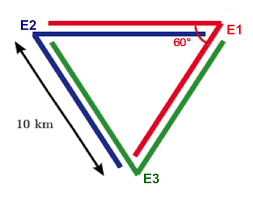
\includegraphics[height=3cm]{figs/gr_qc_12013563.png}};
   \node (img1 )[anchor=center,scale=1,opacity=1] at ([shift={(0.4cm,-2.5cm)}]current page.center) {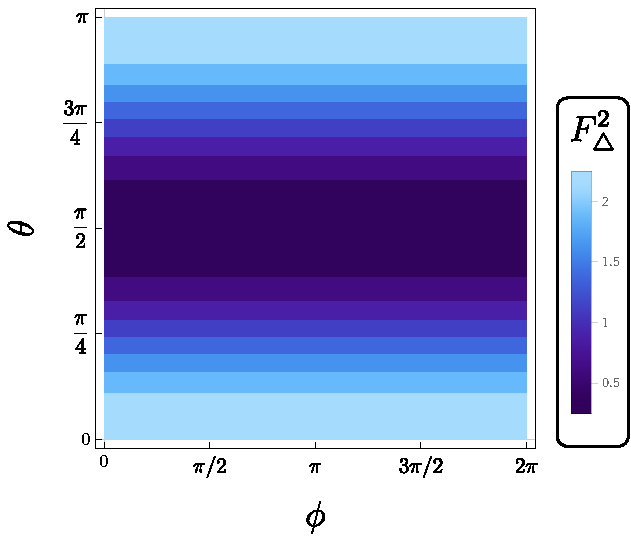
\includegraphics[height=4cm]{../Figures/ET_no_blind_spots.pdf}};
   \node[anchor=center,scale=0.5,opacity=1] at ([shift={(5cm,0.4cm)}]current page.center) {Phys. Rev. D 86, 122001 };
  \end{tikzpicture}

   
\end{frame}


\begin{frame}{Detection criteria}{Optimal Signal-to-Noise Ratio {\bf SNR}}
\vspace{-5mm}
\begin{footnotesize} 
\[
 \rho=\left[ \int_0^\infty d\ln f\, \f{|\red{2\tilde{h}(f)\sqrt{f}}|^2}{S_n(f)}\right]^{1/2} 
\]
\\
\end{footnotesize}
$\sqrt{S_n(f)}\equiv$ {\it amplitude spectral density} ({\bf ASD}) or  detector noise

For compact binary inspirals, $\tilde{h}(f) \sqrt{f} \sim f^{-7/6} f^{1/2} = \red{f^{-2/3}}$
\begin{footnotesize} 
\[
 \rho^2 =  (2A)^2 h_0^2 |Q(\theta,\phi,\psi,\iota)|^2 \int_0^{\bl{f_\text{ISCO}}} df \f{f^{-7/3}}{S_n(f)} 
\]
\end{footnotesize}
%
RMS \red{average} over the angles $ \langle \ldots \rangle \equiv \int \sin\theta d\theta d\phi \int d\psi \int\sin\iota d\iota $
\begin{footnotesize} 
\[
 \langle |Q(\theta,\phi,\psi,\iota)|^2 \rangle_\llcorner = \f{4}{25}, \qquad \langle |Q(\theta,\phi,\psi,\iota)|^2 \rangle_\triangle = \f{9}{25}
\]
\end{footnotesize}
Our Network: \red{three L}-IFOs: 
\begin{footnotesize} 
\begin{align*}
\rho_\text{tot} &= \left[{\sum_{i=1}^3 \rho^2_i}\right]^{1/2} =\left[ \rho_h^2 + \rho_m^2 + \rho^2_l \right]^{1/2} 
	= \boxed{\rho_c\left[\tilde{A}_h^2 + \tilde{A}_m^2 + \tilde{A}_l^2 \right]^{1/2}}\\
\rho_c &\equiv 2 h_0 \left[ \int_0^{{f_\text{ISCO}}} df \f{f^{-7/3}}{S_n(f)}  \right]^{1/2}, \quad \tilde{A}_h = \tfrac{4}{5}A, \quad \tilde{A}_m =\tfrac{2}{5}A, \quad \tilde{A}_l  < \tfrac{\tilde{A}_m}{2}
\end{align*}
\end{footnotesize}
%
\begin{tikzpicture}[overlay,remember picture]
\node[draw, red,thick,minimum width=4.5cm,minimum height=1.25cm] (b) at (3.3,0.7){};
\end{tikzpicture}
%
% 
\end{frame}

\begin{frame}{Detection criteria}{Triangular topology SNR}
%\vspace{-5mm}
\red{Three V-}IFOs
\begin{footnotesize} 
\[
 \rho^2_{\text{tot},\bigtriangleup} = \sum_{A=1}^3 \left(\rho^A\right)^2  =  4 A^2 h_0^2\,|Q(\theta,\phi,\psi,\iota)|_\bigtriangleup^2 \int_0^{f_\text{ISCO}} d f\, \f{f^{-7/3}}{S_n(f)} \,
\]
\end{footnotesize}
\\
Use \bl{RMS-averaged} $|Q|^2$
\begin{footnotesize}
\begin{align*}
\rho_{\text{tot},\bigtriangleup} &= \left[ \int_0^\infty d\ln f\, \f{|{2\tilde{H}_\bigtriangleup(f)\sqrt{f}}|^2}{S_n(f)}\right]^{1/2} 
=\f{6}{5}A\, h_0 \left[\int_0^{f_\text{ISCO}} d f\, \f{f^{-7/3}}{S_n(f)}\right]^{1/2} \\
\end{align*}
\end{footnotesize}
\\
where \begin{small}$\tilde{H}_\bigtriangleup(f)\equiv A\,  \langle |Q|^2_\bigtriangleup\rangle\, h_0 f^{-7/6}= \f{3}{5} A h_0 f^{-7/6}$ \end{small}\\
\vspace{2mm}
Compare with three-L network's \begin{small}$\rho_\text{tot} \approx \tfrac{4}{5}A\, h_0 \left[ \int df \ldots \right]^{1/2} $ \end{small}
%
%
\begin{tikzpicture}[overlay,remember picture]
\node[draw, red,thick,minimum width=4.5cm,minimum height=1.25cm] (b) at (-0.2,2.5){};
\end{tikzpicture}
%
% 
\end{frame}




\begin{frame}{Supplement 1: mode suppression}
\begin{itemize}
 \item For $q=1$ due to symmetry only (2,2), (3,2), (4,2), (4,4) are nonzero 
 \item For $q\ne 1$ all $\ell \ge 2$ modes exist, but are much smaller than $(2,2)$
\end{itemize}
\end{frame}


\begin{frame}{Supplement 2: The expression for $h_c(t)$}
Maggiore chapters 1, 3 and 4
\begin{itemize}
 \item Eq. (3.3) expanded to (3.9), (3.14) to (3.34) to (3.55) to (3.59)
 \item Eq. (3.72): $h(t)$ as angular distribution with mass moments $\ddot{M}_{ij}$'s
 \item At that point we get the scaling $h \sim \tfrac{1}{D}\tfrac{G}{c^4}\ddot{Q}_{ij}$.
 \item Eq. (3.275) shows it expanded in tensor harmonics so up to $\partial^2 Y^{\ell m}$
\end{itemize}
\end{frame}

\begin{frame}{Supp: coord. vs. proper distance in TT gauge}
  Geodesic deviation 
  \[
   \frac{D^2 \xi^\alpha}{D\tau^2} = -R^\alpha_{\beta \gamma\delta}\, \xi^\gamma u^\beta u^\delta 
  \]
In TT gauge,\qquad  $\Longrightarrow \quad\left.\tfrac{d^2 \xi^i}{d\tau^2}\right|_{\tau=0} = -\left. \dot{h}_{ij} \tfrac{d\xi^i}{d\tau}\right|_{\tau=0}$\\
i.e., if mirrors are initially at rest w.r.t to each other ( $\left. \tfrac{d\xi^i}{d\tau}\right|_{\tau=0} =0$ )\\
then $\tfrac{d^2 \xi^i}{d\tau^2}=0\quad \forall t$ \\
$\Longrightarrow$ coordinate separation $\xi^i = \text{constant}$ for all time \\
BUT, proper distance is NOT! \\
Consider mirrors at $\mathbf{x}=x_1$ and at $\mathbf{x}=x_2=x_1+\mathbf{\xi}$
\begin{align*}
  s = \int_1^2 \tfrac{ds}{dx}dx &= (x_2-x_1) \left[ 1 + h_+ \cos(\omega\t)\right]^{1/2} \\
			      & \approx L \left[ 1+\tfrac{1}{2} h_+ \cos\omega t \right] 
\end{align*}
 \end{frame}



\begin{frame}{Supplement 3: Direction of GW emission}
 Mostly off the orbital plane and slightly forward
 \begin{itemize}
  \item Eqs. (3.337-3.338) and Fig. 3.7 show that $\tfrac{d\dot{E}}{d\Omega}$ is max at the poles
  \item Eqs. (4.347), (4.348) with Fig. 4.24 (page 228) show that even for $v=0.99$ the beaming
  is much less significant compared to EM beaming shown in Fig. 4.23.
 \end{itemize}

\end{frame}


\begin{frame}{Supplemet 5: Mass-inclination degeneracy}
 
\end{frame}








\end{document}


